\setcounter{ex}{0}
\begin{ex}%[Cau 1]
$A$  $B$  $f(x)=x^3-3x^2+m$ $m\neq0$.  $m$  $OAB$  $3x+3y-8=0$.
\choice
{\True $m=5$}
{$m=2$}
{$m=6$}
{$m=4$}
\loigiai{
{\bf bgf 1}

   $f'(x)=3x^2-6x=0\iff\hoac{x=0&\implies y=2\\ x=2&\implies y=m-4}\implies A(0;2),~B(2;m-4)$
 
  $G$  $\triangle OAB$,  $G\left(\frac23;\frac{2(m-2)}3\right)$
 
 $G$  $3x+3y-8=0\iff 2+2(m-2)-8=0\iff m=5$
 \\ {\bf ex 2}

  $M(x_o;y_o)$  $AB$. 
 
  $f''(x_o)=0\iff 6x_o-6=0\iff x_o=1\implies y_o=m-2\implies M(1;m-2)$
 
  $G$  $\triangle OAB$,  $\vec{OG}=\frac23\vec{OM}=\left(\frac23;\frac{2(m-2)}3\right)$
 
 $G$  $3x+3y-8=0\iff 2+2(m-2)-8=0\iff m=5$
}

\end{ex}

\begin{ex}%[Cau 2]
 $y=f(x)$ 
\immini{ bla bla ...
\choice[2]
{$(1; 3)$}
{$(3; 1)$}
{\True $(-1; -1)$}
{$(1; -1)$}
}{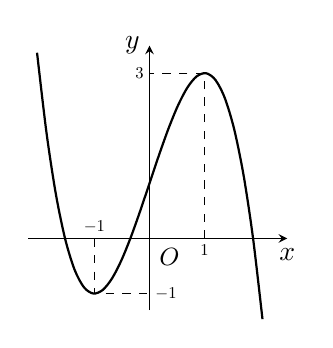
\begin{tikzpicture}[scale=.7]
\draw[-stealth] (-2.2,0) -- (2.5,0) node[below]{$x$};
\draw[-stealth] (0,-1.3) -- (0,3.5) node[left]{$y$};
\draw (0,0) node[below right]{\small $O$};
\draw[dashed] (-1,0)|-(0,-1)(1,0)|-(0,3);
\draw[thick,smooth] plot[domain=-2.04:2.05](\x,{-(\x)^3+3*(\x)+1});
\path(1,0)node[below,scale=.6]{$1$} (-1,0)node[above,scale=.6]{$-1$}
(0,-1)node[right,scale=.6]{$-1$} (0,3)node[left,scale=.6]{$3$};
\end{tikzpicture}}
\loigiai{
bla bla lbla ldl ....... $(-1;-1)$
}
\end{ex}
